\let\negmedspace\undefined
\let\negthickspace\undefined
\documentclass[journal,12pt,onecolumn]{IEEEtran}
\usepackage{cite}
\usepackage{amsmath,amssymb,amsfonts,amsthm}
\usepackage{algorithmic}
\usepackage{graphicx}
\graphicspath{{./figs/}}
\usepackage{textcomp}
\usepackage{xcolor}
\usepackage{txfonts}
\usepackage{listings}
\usepackage{enumitem}
\usepackage{mathtools}
\usepackage{gensymb}
\usepackage{comment}
\usepackage{caption}
\usepackage[breaklinks=true]{hyperref}
\usepackage{tkz-euclide} 
\usepackage{listings}
\usepackage{gvv}                                        
%\def\inputGnumericTable{}                                 
\usepackage[latin1]{inputenc}     
\usepackage{xparse}
\usepackage{color}                                            
\usepackage{array}
\usepackage{longtable}                                       
\usepackage{calc}                                             
\usepackage{multirow}
\usepackage{multicol}
\usepackage{hhline}                                           
\usepackage{ifthen}                                           
\usepackage{lscape}
\usepackage{tabularx}
\usepackage{array}
\usepackage{float}
\newtheorem{theorem}{Theorem}[section]
\newtheorem{problem}{Problem}
\newtheorem{proposition}{Proposition}[section]
\newtheorem{lemma}{Lemma}[section]
\newtheorem{corollary}[theorem]{Corollary}
\newtheorem{example}{Example}[section]
\newtheorem{definition}[problem]{Definition}
\newcommand{\BEQA}{\begin{eqnarray}}
\newcommand{\EEQA}{\end{eqnarray}}
\newcommand{\define}{\stackrel{\triangle}{=}}
\theoremstyle{remark}
\newtheorem{rem}{Remark}

\begin{document}

\title{12.589}
\author{ee25btech11056 - Suraj.N}
\maketitle
\renewcommand{\thefigure}{\theenumi}
\renewcommand{\thetable}{\theenumi}

\begin{document}

\textbf{Question :} Solve the system of equations and find the condition for which the system has \textbf{no solution}:

\begin{align*}
x+y+z &= 6 \\
x+4y+6z &= 20 \\
x+4y+\lambda z &= \mu
\end{align*}

\textbf{Solution :}

\begin{table}[h!]
  \centering
  \begin{tabular}{|c|c|}
\hline
\textbf{Name} & \textbf{Value} \\ \hline
$\vec{A}$ & $\myvec{2 & 1 \\0 & 3}$ \\ \hline
\end{tabular}

  \caption*{Table : Equations}
  \label{12.589}
\end{table}

The system of equations in matrix form is :
\begin{align}
\myvec{1 & 1 & 1\\1 & 4 & 6\\1 & 4 & \lambda}\myvec{x\\y\\z} &= \myvec{6\\20\\\mu}
\end{align}

Forming the augmented matrix,
\begin{align}
\myaugvec{3}{1 & 1 & 1 & 6\\1 & 4 & 6 & 20\\1 & 4 & \lambda & \mu}
\end{align}

Using Gaussian elimination,
\begin{align}
\myaugvec{3}{1 & 1 & 1 & 6\\1 & 4 & 6 & 20\\1 & 4 & \lambda & \mu}
\xleftrightarrow[\;R_2 \to R_2 - R_1\;]{\;R_3 \to R_3 - R_1}
\myaugvec{3}{1 & 1 & 1 & 6\\0 & 3 & 5 & 14\\0 & 3 & \lambda-1 & \mu-6}
\end{align}

\begin{align}
\myaugvec{3}{1 & 1 & 1 & 6\\0 & 3 & 5 & 14\\0 & 3 & \lambda-1 & \mu-6}
\xleftrightarrow{R_3 \to R_3 - R_2}
\myaugvec{3}{1 & 1 & 1 & 6\\0 & 3 & 5 & 14\\0 & 0 & \lambda-6 & \mu-20}
\end{align}

From back substitution we get:
\begin{align}
(\lambda-6)z &= \mu-20
\end{align}

For the system to have \textbf{no solution}, we must have
\begin{align}
  \lambda &= 6 & \mu \neq 20
\end{align}

So, we get zero equal to a non-zero value which is not possible .\\
Therefore the system of equations has \textbf{no solution}.

\textbf{Final Answer :} The system has no solution when $\lambda=6$ and $\mu \neq 20$.

\pagebreak

\begin{figure}[h!]
  \centering
  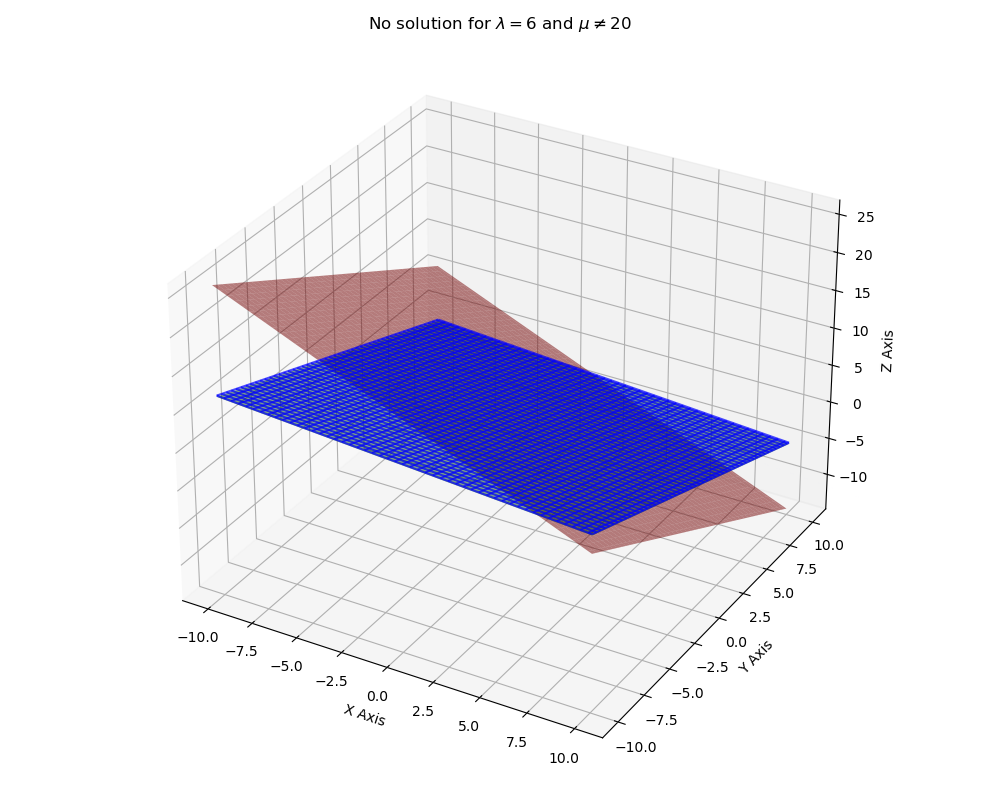
\includegraphics[width=0.7\columnwidth]{figs/planes.png} 
   \caption*{Fig : Planes}
  \label{Fig1}
\end{figure}

\end{document}

